This section reviews research on emergency decision-support systems, smart-city sensing, and emergency vehicle routing in the context of fire response. Although prior work has improved situational awareness and routing efficiency, these approaches are often developed in isolation and lack integration of heterogeneous data, explainability, and governance. This section highlights these gaps and motivates the design of the proposed FireRoute system.

\subsection{Emergency decision-support systems and incident logistics}
Decision-support systems (DSS) for emergency logistics have long focused on supporting rapid decision-making under time pressure and uncertainty~\cite{su142013423}. Prior systems emphasize integrating traffic conditions, incident reports, and operational constraints to improve response efficiency. A common theme in this body of work is the recognition that effective emergency response requires more than shortest-path computation.


However, existing approaches typically treat routing and decision support as loosely coupled components. While they incorporate elements such as traffic dynamics or incident severity, they often do not jointly model infrastructure readiness (e.g., hydrant availability), environmental sensing, and post-incident accountability within a unified workflow~\cite{fi17120574}. As a result, these systems provide partial decision support but fall short of delivering a fully integrated operational pipeline.

\subsection{Smart-city sensing and fire/disaster systems}
Advances in smart-city infrastructure have introduced a wide range of sensing technologies, including IoT-based environmental monitoring, embedded signaling systems, and building-scale safety platforms~\cite{REJEB2022100565}. These systems demonstrate the potential of real-time data to enhance situational awareness during fire and disaster events. In particular, recent work has highlighted the importance of integrating heterogeneous sensor streams and ensuring system reliability in dynamic and uncertain environments~\cite{SUN2026114440}.

Despite these advances, most sensing-driven systems are designed as monitoring or alerting platforms rather than as decision-support engines. Sensor data is frequently presented through dashboards or visualization interfaces, leaving the burden of interpretation and action on human operators~\cite{NAYAK2024783}. The lack of tight integration between sensing layers and routing or dispatch logic limits the operational impact of these systems, as environmental context is not systematically incorporated into decision-making processes.

\subsection{Emergency vehicle routing and dispatch under uncertainty}
The literature on emergency vehicle routing has explored a variety of optimization strategies, including dynamic routing, traffic-aware path planning, and resource allocation under uncertainty. These approaches have improved routing efficiency and responsiveness, particularly in complex urban environments where congestion and stochastic travel conditions play a significant role.

Nevertheless, most routing models remain focused on optimizing travel time or coverage metrics, with limited consideration of infrastructure constraints and environmental degradation. Additionally, routing and dispatch are often treated as separate problems, leading to fragmented solutions that do not capture the full operational chain from responder deployment to incident resolution~\cite{OLADIGBOLU2025118419}. As a consequence, routing outputs may be mathematically optimal but operationally impractical when real-world constraints such as access limitations or asset availability are taken into account.

\subsection{Positioning of FireRoute}

\begin{figure*}[t]
    \centering
    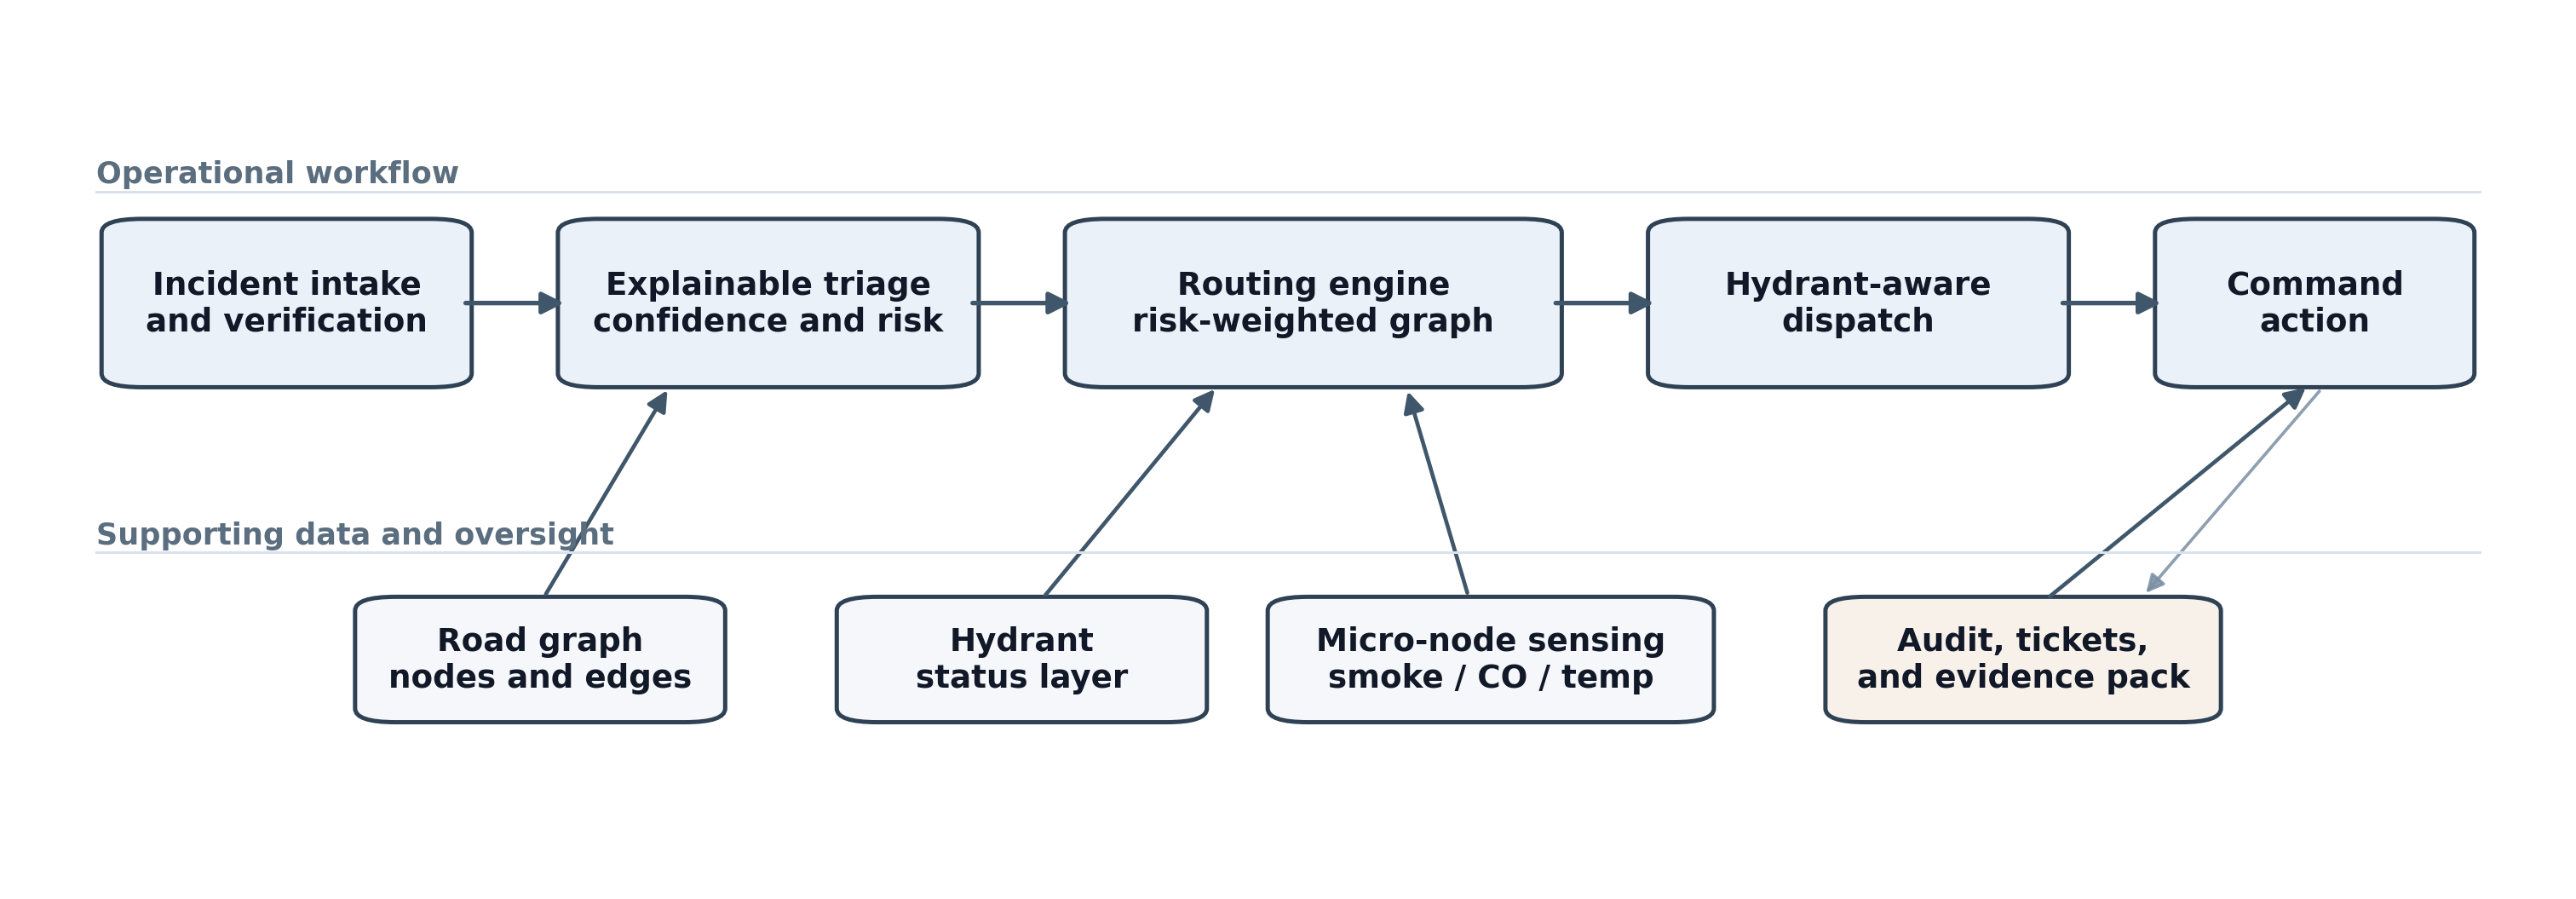
\includegraphics[width=\textwidth]{figure1_architecture}
    \caption{FireRoute architecture integrating incident intake, explainable triage, risk-weighted routing, hydrant-aware dispatch, and evidence-ready governance.}
    \label{fig:architecture}
\end{figure*}

In contrast to prior work, FireRoute is designed as an integrated, service-level decision-support system rather than a routing-only solution. The key distinction lies in its holistic treatment of emergency response as a workflow that connects incident intake, explainable risk assessment, risk-aware routing, hydrant availability, environmental sensing, dispatch actions, and governance outputs within a single architecture.

Rather than optimizing routing in isolation, the system emphasizes operational realism, explainability, and reproducibility. This positioning aligns with emerging directions in intelligent urban systems, where decision support is expected to combine heterogeneous data sources, support human interpretability, and enable accountability through auditable system outputs. By bridging routing, sensing, and governance within a unified framework, FireRoute advances beyond traditional approaches and provides a foundation for next-generation emergency response systems.